
\begin{table}[H]
    \centering
    \hspace*{-1.75cm}
    \begin{tabular}{rc|c|>{\centering\arraybackslash}p{0.5\linewidth}|} 
        \cline{3-4} 
        & Fallabbildung & Bedingungen & Bewertung \\\cline{3-4}
        \vspace{-1.35em} \\ \cline{3-4}
            1&\begin{minipage}{0.25\textwidth}
                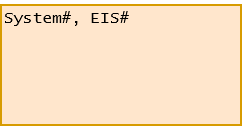
\includegraphics[width=\linewidth]{gfx/IA21.drawio.png} 
            \end{minipage}
            &$\begin{array}{l}
                \scriptstyle EIS\# \;=\; Sys\#; \\
              \end{array}$ 
            &\begin{minipage}{0.5\textwidth} 
                \smaller
                \textit{Standardfall}: Keine große Aussage für \ac{IA} kann jedoch ein System mit sehr vielen Abhängigkeiten identifizieren.
            \end{minipage} 
            \\ \cline{3-4}
            2&\begin{minipage}{0.25\textwidth}
                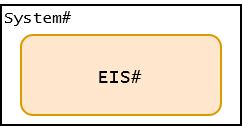
\includegraphics[width=\linewidth]{gfx/IA22.drawio.png} 
            \end{minipage}
            &$\begin{array}{l}
                \scriptstyle |System\#| \;>\; |EIS\#|; \\
                \scriptstyle EIS\# \;\subset\; System\# \\
              \end{array}$ 
            & \begin{minipage}{0.5\textwidth} 
                \smaller
                \textit{Verbesserter Fall}: Die geschätzte Änderung betrifft nicht das gesamte System und kann genauer definiert werden.
            \end{minipage} 
            \\ \cline{3-4}
            3&\begin{minipage}{0.25\textwidth}
                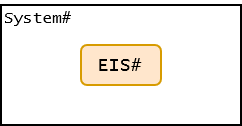
\includegraphics[width=\linewidth]{gfx/IA23.drawio.png} 
            \end{minipage}
            &$\begin{array}{l}
                \scriptstyle |System\#|\; \gg \; |EIS\#|; \\
                \scriptstyle EIS\# \;\subset\; System\# \\
              \end{array}$ 
            & \begin{minipage}{0.5\textwidth}
                \smaller
                \textit{Optimalfall}: Geschätzte Änderung beschränkt sich auf eine relativ kleine Untermenge des Systems.
            \end{minipage} 
            \\ \cline{3-4}
        \cline{3-4}
    \end{tabular}
    \caption{Mögliche \acsfont{EIS\#}/\acsfont{System\#} Abhängigkeiten nach Arnold et al. \cite[297]{app_bohner}}
    [Eigene Darstellungen]
    \label{tab:eis_sys}
\end{table}
